\begin{figure}[t]
\centering
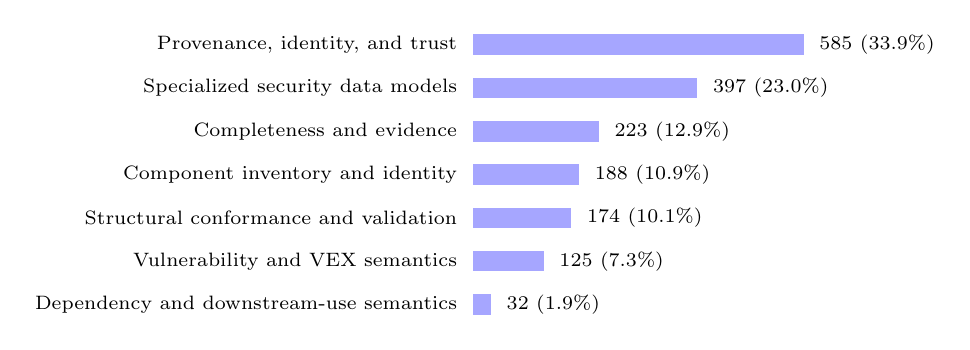
\begin{tikzpicture}[x=1cm,y=1cm]
\scriptsize
\node[anchor=east] at (0,0.00) {Provenance, identity, and trust};
\fill[blue!35] (0.10,-0.13) rectangle (4.30,0.13);
\node[anchor=west] at (4.40,0.00) {585 (33.9\%)};
\node[anchor=east] at (0,-0.55) {Specialized security data models};
\fill[blue!35] (0.10,-0.68) rectangle (2.95,-0.42);
\node[anchor=west] at (3.05,-0.55) {397 (23.0\%)};
\node[anchor=east] at (0,-1.10) {Completeness and evidence};
\fill[blue!35] (0.10,-1.23) rectangle (1.70,-0.97);
\node[anchor=west] at (1.80,-1.10) {223 (12.9\%)};
\node[anchor=east] at (0,-1.65) {Component inventory and identity};
\fill[blue!35] (0.10,-1.78) rectangle (1.45,-1.52);
\node[anchor=west] at (1.55,-1.65) {188 (10.9\%)};
\node[anchor=east] at (0,-2.20) {Structural conformance and validation};
\fill[blue!35] (0.10,-2.33) rectangle (1.35,-2.07);
\node[anchor=west] at (1.45,-2.20) {174 (10.1\%)};
\node[anchor=east] at (0,-2.75) {Vulnerability and VEX semantics};
\fill[blue!35] (0.10,-2.88) rectangle (1.00,-2.62);
\node[anchor=west] at (1.10,-2.75) {125 (7.3\%)};
\node[anchor=east] at (0,-3.30) {Dependency and downstream-use semantics};
\fill[blue!35] (0.10,-3.43) rectangle (0.33,-3.17);
\node[anchor=west] at (0.43,-3.30) {32 (1.9\%)};
\end{tikzpicture}
\caption{CycloneDX theme distribution recomputed from 1,724 extracted requirements.}
\label{fig:cdx-theme-distribution}
\end{figure}
